Zu erst wird der Winkel $\phi$ ermittelt. Mit der Gleichung:
\begin{align*}
  \phi=\frac{1}{2}(\phi_R-\phi_L)
\end{align*}
lässt sich aus den Messwerten $\phi$ berechnen.
Die Messwerte und die jeweiligen $\phi$ sind in der Tabelle \ref{tab:phi} aufgeführt
Der Mittelwert von $\phi$ ergiebt sich zu:
\begin{align*}
  \phi_m=\SI{60,02\pm0,04}{°}
\end{align*}
\begin{table}[h!]
  \centering
  \caption{Messung zur Bestimmung von $\phi$}
  \label{tab:phi}
  \begin{tabular}{c c c}
    \toprule
      $\phi_L$/° & $\phi_R$/°  & $\phi$/° \\
    \midrule


90,9	&211,0	&60,05\\
93,4	&213,4	&60,00\\
95,9	&216,1	&60,10\\
92,7	&212,7	&60,00\\
95,3	&215,4	&60,05\\
95,7	&215,7	&60,00\\
95,3	&215,2	&59,95\\


    \bottomrule
  \end{tabular}
\end{table}



Berechnung des Brechungsindex n aus $\phi$ und $\eta$ in Abhängigkeit von der Wellenlänge.
$\eta$ berechnet sich wie folgt:
\begin{align*}
  \eta=180-(\Omega_R-\Omega_L)
\end{align*}
Mit der Formel:
\begin{align*}
  \text{n}=\frac{\text{sin}\frac{\eta+\phi}{2}}{\text{sin}\frac{\phi}{2}}
\end{align*}
wird der Brechungsindex n berechnet.
In der Tabelle \ref{tab:nu} sind die Messwerte und die errechneten Ergebnisse aufgeführt.
\begin{table}[h!]
  \centering
  \caption{Messung zur Bestimmung von n}
  \label{tab:nu}
  \begin{tabular}{c c c c c c}
    \toprule
      $\lambda$ & $\lambda$/nm & $\Omega_R$/° & $\Omega_L$/°  & $\eta$/° & $\text{n}(\lambda_i)$\\
    \midrule





Rot	        & 643.84 &215,5	&94,5	&59,0 & 1,722\\
Orange	    & 576.96 &215,8	&94,8	&59,0 & 1,722\\
Gelb	      & 546.07 &215,7	&95,0	&59,3 & 1,725\\
Grün	      & 508.58 &215,3	&95,5	&60,2 & 1,733\\
Blau	      & 479.99 &214,9	&96,0	&61,1 & 1,741\\
Dunkelblau	& 467.81 &214,7	&96,2	&61,5 & 1,744\\
Lila	      & 453.83 &214,2	&96,8	&62,6 & 1,753\\












    \bottomrule
  \end{tabular}
\end{table}


Die Wertepaare ($\text{n}^2$, $\lambda$) werden in der Graphik $\ref{fig:dis}$ aufgetragen.
\begin{figure}
  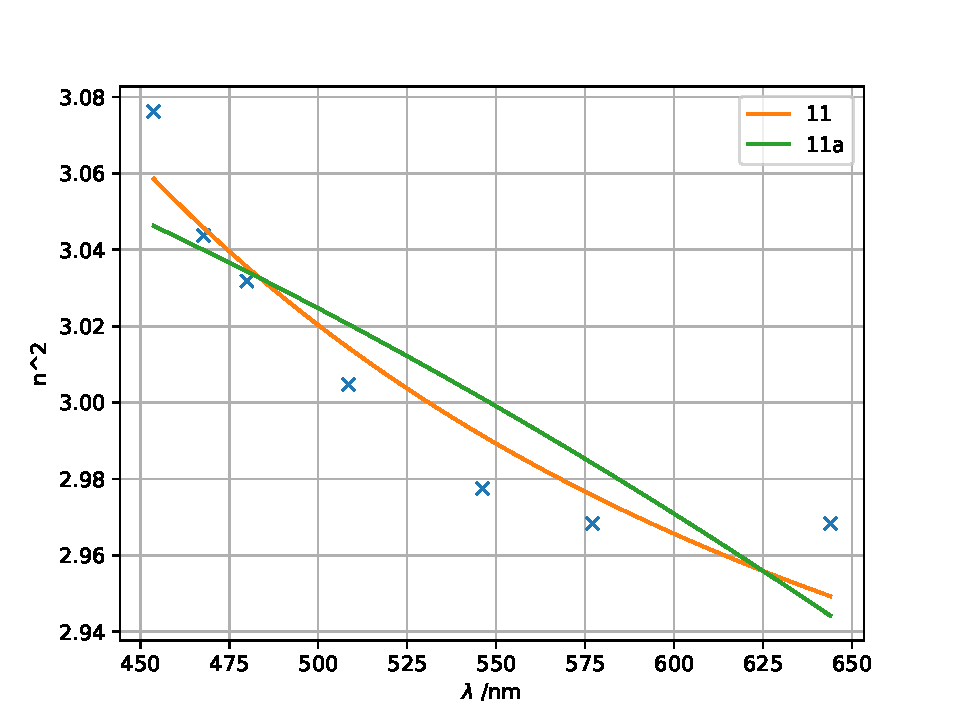
\includegraphics{Dispersionskurve.pdf}
  \caption{Dispersionskurve}
  \label{fig:dis}
\end{figure}
Es werden die beiden Funktionen:
\begin{align}
  \text{n}^2(\lambda)=A_0+\frac{A_2}{\lambda^2}
  \label{eqn:n}
\end{align}
und
\begin{align*}
  \text{n}^2(\lambda)=A'_0-A'_2\cdot\lambda^2
\end{align*}
an die Wertepaare gefittet.

Daraus ergeben sich die Werte:
\begin{align*}
  A_0&=(2,8414\pm0,0006 )\\
  A_2&=(4,4716\pm4342,2614)\cdot10^4\\\\
  A'_0&=(3,1471 \pm0,0013)\\
  A'_2&=(4,8921\pm0,0000001)\cdot10^{-7}\\
\end{align*}

Über die Formeln:
\begin{align}
  s^2_{\text{n}}=\frac{1}{z-2}\sum_{i=1}^z\left(\text{n}^2(\lambda_i)-A_0-\frac{A_2}{(\lambda_i)^2}\right)^2
  \label{eqn:s}
\end{align}

\begin{align*}
  s^2_{\text{n}'}=\frac{1}{z-2}\sum_{i=1}^z\left(\text{n}^2(\lambda_i)-A'_0+A'_2\cdot(\lambda_i)^2\right)^2
\end{align*}
kann die Summe der jeweiligen Abweichungsquadrate bestimmt werden um die geeignetere Formel zu ermitteln.
Die Abweichungsquadrate berechnen sich zu:
\begin{align*}
  s^2_{\text{n}}&=0,0002\\
  s^2_{\text{n}'}&=0,0005
\end{align*}
Das Abweichungsquadrat der Formel \ref{eqn:s} ist geringer daher wird die Funktion \ref{eqn:n} verwendet.
Schon in der Graphik \ref{fig:dis} ist zu erkennen, dass die Funktion \ref{eqn:n} besser zu den Messwerten passt.\\
Nun wird die Abersche Zahl bestimmt. Diese ist läst sich berechnen durch:
\begin{align*}
  v:=\frac{\text{n}_\text{D}-1}{\text{n}_\text{F}-\text{n}_\text{C}}
\end{align*}
$\text{n}_\text{D}, \text{n}_\text{F}, \text{n}_\text{C}$ sind die Brechungsindices für bestimmte Wellenlängen die sich aus der Funktion \ref{eqn:n} ergeben.
\begin{align*}
\text{n}_\text{C}&=1,716&&\lambda_\text{C}=656\\
\text{n}_\text{D}&=1,723&&\lambda_\text{D}=589\\
\text{n}_\text{F}&=1,741&&\lambda_\text{F}=486\\
\end{align*}
Mit den Werten lässt sich $v$ berechnen zu:
\begin{align*}
  v=29,28
\end{align*}
Das Auflösungsvermögen läst sich mit
\begin{align*}
  A:=\frac{\lambda}{\Delta\lambda}=\text{b}\frac{d\text{n}(\lambda)}{d\lambda}=\text{b}\frac{A_2}{\lambda^3\cdot\sqrt{A_0+\frac{A_2}{\lambda^2}}}
\end{align*}
bestimmen zu:
\begin{align*}
  A:=\SI{0,0005}{nm}
\end{align*}
$\lambda$ ist dabei die mittlere Wellenlänge.

Die Absorptionsstelle $\lambda_1$ wird aus der Formel \ref{eqn:größer} hergeleitet und berechnet sich nach
\begin{align*}
  \lambda_1=\sqrt{\frac{A_2}{A_0-1}}.
\end{align*}
Die Absorptionsstelle liegt bei:
\begin{align*}
  \lambda_1=\SI{125,44}{nm}
\end{align*}
